\subsection{Umweltbelastung durch \ce{CO2} Ausstoß}
\lfoot{Autor: Hüseyin Bozkurt}

\subsubsection{Definition und Entstehung}
Kohlenstoffdioxid (\ce{CO2}) ist ein unsichtbares, geruchsloses Gas bestehend aus einem Kohlenstoff und zwei Sauerstoff-Atomen. 
In jedem Stoffwechselprozess spielt Kohlenstoffdioxid eine wichtige Rolle, da beispielsweise der Mensch \ce{CO2} ausatmet. 
Bei vielen Energiegewinnungsverfahren werden durch Verbrennung Energien freigesetzt, die als Nebenprodukt Kohlenstoff produzieren. 
In der freien Luft verbinden sich diese Kohlenstoffpartikel mit Sauerstoff zu \ce{CO2}.
\ce{CO2} ist Reaktionsträge und besitzt keine giftige Eigenschaft. 
Das Problem mit den Unmengen an ausgestoßenem \ce{CO2} ist, dass sein massives Vorkommen die Atmosphäre beschädigt.

Alle Fahrzeuge, die fossile Brennstoffe als Energiequelle nutzen 
(wie zum Beispiel Diesel, Flüssiggas, Benzin und auch Biotreibstoff), erzeugen Kohlenstoff als Abgas. 
Indem der Motor den Kraftstoff zusammen mit Luftsauerstoff verbrennt, gelangt das \ce{CO2} über die Abgasanlage in die Atmosphäre. 
Eine effektive Methode zur Beseitigung der Kohlenstoffpartikel gibt es zurzeit nicht. 
Der benutzte Kraftstoff bestimmt, wie viel \ce{CO2} bei der Verbrennung als Nebenprodukt entsteht.
Beispielsweise entsteht bei der Verbrennung von einem Liter Diesel mehr Kohlenstoffdioxid, als bei einem Liter Benzin.
Der Kraftstoffverbrauch eines Kraftfahrzeugs und sein \ce{CO2}-Ausstoß stehen daher in enger Verbindung.
Demnach existieren Werte, die man als Grenze für den Verbrauch festlegen kann. 
Heutzutage spricht man von der Einheit Gramm pro Kilometer [g/km] als normierte Verbrauchsmessung.
Der Lenker eines PKW hat Einfluss auf seinen \ce{CO2}-Ausstoß, indem dieser bei starken und überflüssigen Beschleunigungsmanövern
zu diesem Zeitpunkt mehr Schadstoffe produziert als nötig.
Mit diesem Diplomprojekt, wollen wir Fahrenden ein Werkzeug in die Hand geben, ihren \ce{CO2}-Ausstoß während und nach der Fahrt
einschätzen zu können. Damit haben sie die Möglichkeit ihre Fahrweise in Hinblick auf den \ce{CO2}-Ausstoß zu verbessern.

\clearpage

\subsubsection{Treibhauseffekt}
\ce{CO2} gilt als eines der häufigsten Treibhausgase.
Das Kohlenstoffdioxid steigt bis zur Atmosphäre auf und bildet dort eine \textit{Mauer}.
Sonnenstrahlen können zwar ohne weiteres durch, doch nicht so leicht wieder raus. Das heisst, dass die Sonnenstrahlen,
die von der Erdoberfläche wieder zurück in den Weltraum reflektiert werden sollten, von der Erdatmosphäre zurück auf die Erde geworfen werden.
Der Treibhauseffekt gilt als eine der Hauptursachen für den Klimawandel, welcher drastische Folgen für Natur, Tiere und Menschen hat. 
Zu viel \ce{CO2} in der Atmosphäre bringt unter anderem das Abschmelzen von Gletschern, 
den Anstieg der Meerestemperatur, den Anstieg des Meeresspiegels, 
Aussterben von Pflanzen und Tieren und Wetterphänomene wie zum Beispiel sehr warme Winter, Stürme etc.

\begin{figure}[!htb]\centering
	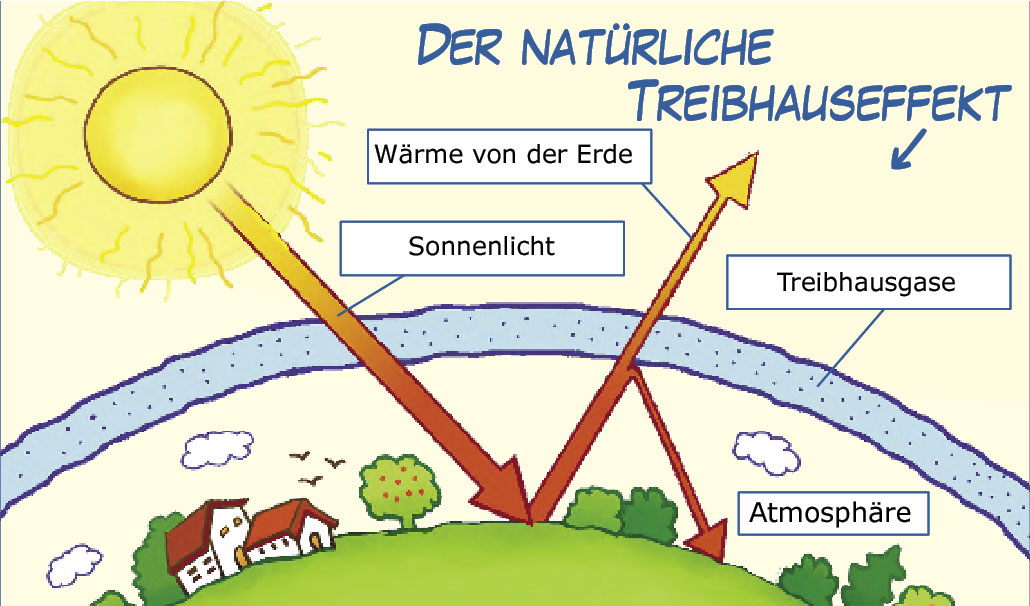
\includegraphics[width=0.6\textwidth]{images/treibhaus1}
	\caption{Der Treibhauseffekt \cite{BOZH.ch1-co2-umwelt.treibhaus1}}
\end{figure}
 
\subsubsection{Das Kyoto-Protokoll}
Im Rahmen des Kyoto-Protokolls haben sich viele westliche Staaten zu einer Reduktion der Treibhausgase verpflichtet. 
Dieses Protokoll war der Startschuss für die Suche nach erneuerbaren Energien. 
Anfang 2015 sind Gesetzesregelungen in Kraft getreten, die den Durchschnittsverbrauch eines PKW auf 130g/\ce{CO2} pro kilometer limitierten. 
Bis 2020 soll dieses Limit auf 95g/CO2 pro kilometer herunter gesetzt werden.

\clearpage